\documentclass[10pt,twocolumn,a4j]{jsarticle}
\usepackage[dvipdfmx]{graphicx} %図等のパッケージ
\usepackage{amsmath} %数式系のパッケージ
\usepackage{amssymb}
\usepackage{cases} %case用パッケージ
\usepackage{authblk}
\usepackage{multirow}%ggr
\usepackage[top=10mm, bottom=5mm, left=15mm, right=15mm]{geometry}
\renewcommand{\baselinestretch}{0.70}
\bibliographystyle{junsrt}
\bibliographystyle{unsrt}
\makeatletter
\newcommand{\figcaption}[1]{\def\@captype{figure}\caption{#1}}
\newcommand{\tblcaption}[1]{\def\@captype{table}\caption{#1}}
\makeatother
\usepackage{subfigure}
\usepackage{here}
\pagestyle{empty}


\begin{document}
\title{青斑核活動の非対称性に着目したADHDの瞳孔径制御モデルの構築}
\author{(指導教員 信川 創 准教授) 

信川研究室 1831053番 熊野 開}
\date{}

\maketitle


\section{はじめに}
注意欠陥/多動性障害 (Attention Deficit Hyperactivity Disorder : ADHD) は,不注意,衝動性,および多動性を特徴とする神経発達障害である.
ADHDの症状は成人になるにつれて,多動性と衝動性があまり目立たなくなる.したがって,成人のADHDの症状を検出することは,子供よりも困難である.

ADHD患者と健常者の違いを調べるために,脳の神経活動の比較が行われており,特に覚醒と注意に重要な役割を果たすノルアドレナリン(NA)神経経路の起点である青斑核(Locus ceruleus : LC)の過活動が原因であることが明らかになっている\cite{rowe2005biophysical}.

LC活動を推定するために,瞳孔径の挙動が注目されている.
近年の研究では,瞳孔径の挙動が,覚醒や注意などの ADHD に関連する認知機能に関わる神経活動を反映していることが明らかとなった\cite{rajkowski1993correlations}.
したがって,瞳孔径は,いくつかの精神障害における注意機能と覚醒機能の機能障害を示している可能性がある.

異常なLC活動を検出するために,
瞳孔径の挙動によって推定された神経活動を利用して,瞳孔径の複雑な時間的パターンと
両眼の瞳孔径の非対称性に焦点を当てた研究が行われている.
Poynter は,瞳孔の非対称性が注意力の負荷,および不注意や多動性という ADHD の症状を反映していることを示した\cite{poynter2017pupil}.
さらにLiu らによる瞳孔制御神経経路の最近の研究では, LC からの副交感神経経路は,
以前考えられていた同側部分に加えて,エディンガー・ウェストファル核 (EWN) の同側および対側の両方の部分に抑制的に投射し,
瞳孔括約筋を制御することが明らかになった\cite{liu2017dynamic}.
この成果により,瞳孔径挙動とLC活動の関係性,特に瞳孔径挙動の対称性についての起源が解明されつつある\cite{liu2017dynamic}.

LCを起源とする神経経路からの瞳孔径挙動のメカニズムと,覚醒機能および注意機能との関係を説明するために,瞳孔径を制御する神経系の数学的モデルが提案されている.
最近では,Nobukawa らが LCから EWNへの新たに発見された対側投影に焦点を当てた瞳孔径の制御モデルの作成を行った.
このモデルは,瞳孔径の時間的挙動の複雑さと対称性が非線形の決定論的なプロセスを反映していることを明らかにした\cite{10.3389/fphys.2021.614479}.

ADHDの瞳孔径の複雑さと対称性の研究が行われている\cite{nobukawa2021identification}.
しかし,ADHDの特徴であるLCの過活性と非対称性が瞳孔径にどのような影響を与えるかはモデルベースの解析が必要であるが,そのような研究は未だ行われていない.
そこで,そのようなADHDの瞳孔径制御モデルを作成すれば,瞳孔径の挙動からADHDの LC活動の推定が実現出来るという仮説を立てた.
本研究では, LCから EWNへの反対側の投影を組み込んだ瞳孔径制御モデルに対して, 
LCの過活動及び右半球の LCの機能障害を反映させた瞳孔径モデルを構築し,仮説の検証を行う.
具体的には,瞳孔径の時間の複雑さの尺度として,サンプルエントロピー(Sample Entoropy : SampEn)を分析した.


\section{手法}
\subsection{瞳孔径分析 : 複雑性}
瞳孔径の時間的な複雑さを定量化するために, SampEnを計算した.
$m$次元のベクトルは, $n$個の確率変数を $z$スコアで正規化されたもので構築される.これを (\ref{eq1})式で示す.

\begin{equation}
\label{eq1}
x_{i}^{m}=\left\{x_{i}, x_{i+1}, \cdots, x_{i+m-1}\right\}
\end{equation}

また,確率$C_{m}(r)$は$i$と$j(i \neq j, i, j=1,2 \cdots)$のベクトルを使用して計算される.これを(\ref{eq2})式に示す.

\begin{equation}
\label{eq2}
C_{m}(r)=\sum_{i, j \in r, i \neq j} \frac{\left|x_{i}^{m}-x_{j}^{m}\right|}{(N-m+1)(N-m)}
\end{equation}

$\left|x_{i}^{m}-x_{j}^{m}\right|$は$x_{i}^{m}$と$x_{j}^{m}$の2つのベクトルの距離が許容誤差$r$よりも小さい時の数を示している.
SampEnの$h(r,m)$は (\ref{eq3})式で定義される.

\begin{equation}
\label{eq3}
h(r,m)=-\log \frac{c_{m+1}(r)}{c_{m}(r)}
\end{equation}

今回の研究では, $r=0.2,m=2$を使用した.
$h(r,m)$は時系列の複雑さが増加すると,値が増加する.

\subsection{瞳孔径制御の神経モデル}
Liuら(2017) によって発見された LCから EWNへの対側の投影が含まれているモデルを構築する.
LCは全体的に同期する1つの神経細胞集団ではなく,複数の同期的に発火する神経細胞集団で構成されることが明らかになっている.
従って,今回の研究では左と右の LCで異なる神経集団を想定した.
LCのニューロン集団の活動を説明するために,結合されたローレンツモデルを利用した.

LCの神経集団活動$x_\text{i}$($\text{i}=\text{left},\text{right}$)を(\ref{eq13})で示す.

\begin{equation}
\label{eq13}
x_\text{i}=\text { L zscore }\left(x_\text{i}\right)+b_\text{i}
\end{equation}

$L$と$b_\text{i}$はパラメータであり, $b_\text{i}$は LCの発火率を表している.
今回の研究では, $b_\text{left} \neq b_\text{right}$である.zscoreは$z$スコア変換を適用した.
副交感神経経路では, EWNから毛様神経経節への出力$S_\text{left}$と$S_\text{right}$を (\ref{eq15}),(\ref{eq16})式で示す.

\begin{equation}
\label{eq15}
S_\text{left}=f\left(-\omega_\text{left~left} x_\text{left}-\omega_\text{right~left} x_\text{right}+\beta_\text{left}\right)
\end{equation}

\begin{equation}
\label{eq16}
S_\text{right}=f\left(-\omega_\text{right~right} x_\text{right}-\omega_\text{left~right} x_\text{left}+\beta_\text{right}\right)
\end{equation}

$\omega_\text{right~left}$は$\text{LC}_\text{right}$から$\text{EWN}_\text{left}$への抑制のシナプス結合の重み,$\omega_\text{left~right}$は$\text{LC}_\text{left}$から$\text{EWN}_\text{right}$への抑制のシナプス結合の重みである. $\beta_\text{left}$は$\text{EWN}_\text{left}$への他のすべての入力,$\beta_\text{right}$は$\text{EWN}_\text{right}$への他のすべての入力を表している.
ここで活性化関数を (\ref{eq17})式で示す.

\begin{equation}
\label{eq17}
f(x)=\tanh (x)+1
\end{equation}

対側シナプスの重みは$\omega_\text{i}=0.15$に設定した.交感神経経路では,上頚神経節への入力は(\ref{eq18})式で示す.

\begin{equation}
\label{eq18}
D_\text{i}=s_\text{i} x_\text{i}
\end{equation}

$D_\text{i}$は上頚神経節へのLC接続のシナプス荷重を示している.
ここで, $S_\text{i}$と$D_\text{i}$はそれぞれ瞳孔径の散大筋,括約筋の役割を示している.
瞳孔径に散大筋と括約筋の活性化に対応させた式を(\ref{eq20})式で示す.

\begin{equation}
\label{eq20}
P_\text{i}=D_\text{i}-S_\text{i}+P_{0}
\end{equation}

本研究では,$\omega_\text{left~left}=\omega_\text{right~right}=0.3, \omega_\text{left~right}=\omega_\text{right~left}=0.15,s_\text{i}=0.3, \beta_\text{i}=3.5, P_\text{0}=3.0, L=1.5$と設定した.


\section{結果}
瞳孔制御の神経モデルから計算された瞳孔径の変化の複雑性を評価した.図1は左右の瞳孔径から得られたSampEnの差分を示しており,左右瞳孔径での差が,SampEnで$-0.06$から$0.08$(SampEnの最大最小の幅に対して$66.7\%$)を示している.

\begin{figure}[H]
    \centering
     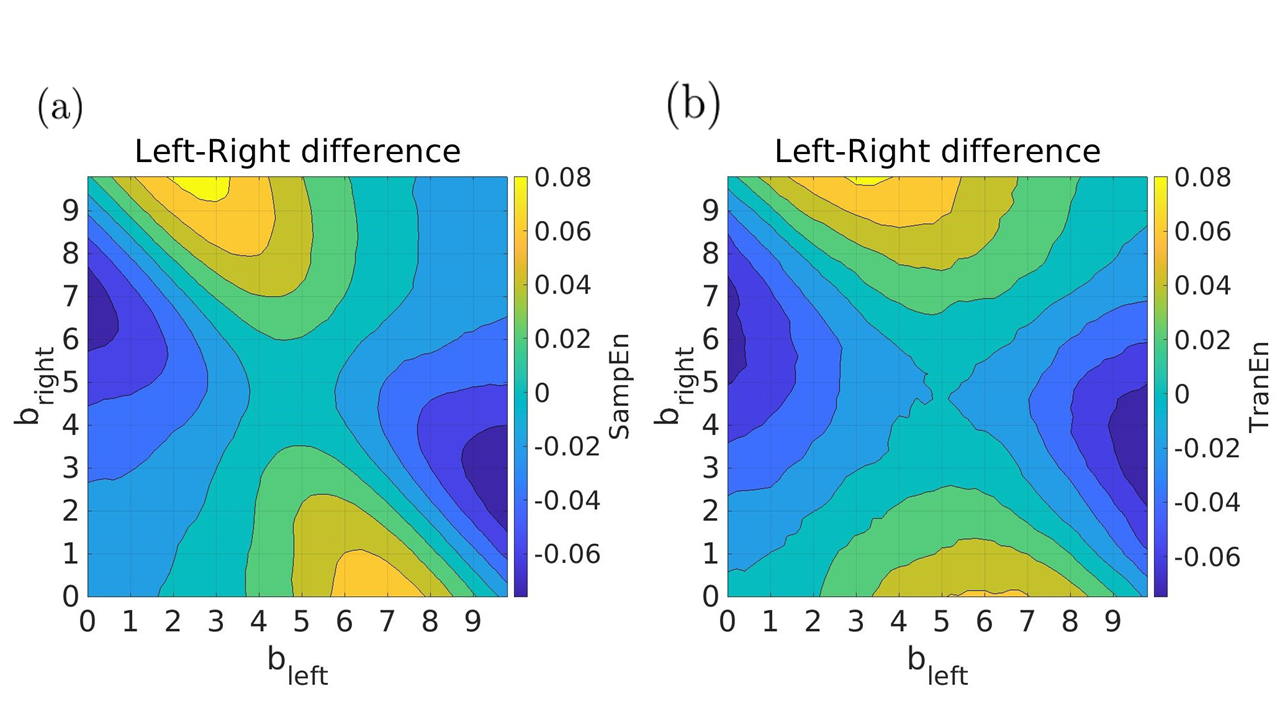
\includegraphics[keepaspectratio, scale=0.27]
      {result.png}
   \caption{左右瞳孔径の複雑性と対称性の差分
   (a)左瞳孔径のSampEnと右瞳孔径のSampEnの差分,
   (b) 左瞳孔径から右瞳孔径へのTranEnと右瞳孔径から左瞳孔径へのTranEnの差分.}
\end{figure}


\section{考察}
本研究では,ADHDの瞳孔径のモデルを構築し,瞳孔径の自律的変化の複雑性の評価を行った.左右瞳孔径の複雑性解析の結果,LC活動の差は,非線形的な複雑性において,瞳孔径の左右差に顕著に表れる領域と左右差が表れない領域が存在していることが明らかとなった.

本研究で得られたこのような左右差の非線形的なプロフィールを持つ複雑性の左右差も,注意機能に関わるLC活動の左右差を反映していると考えられ,これらの特性を取り入れたLCの活動状態の推定に利用できると考えられる.


\section{おわりに}
この研究では,ADHDの瞳孔径制御モデルを構築し,SampEnを使用して,ADHDの瞳孔径のLCの活動,複雑性,及び対称性の関係を明らかにした.
この知見は,ADHDや神経障害に適用するための瞳孔径測定や診断ツールに適用される可能性があると考えられる.

\bibliography{mission}

\end{document}



